\documentclass[11pt, a4paper]{article}
\usepackage[utf8]{inputenc}
\usepackage[left=2.35cm, right=3.35cm, top=3.35cm, bottom=3.0cm]{geometry}
\usepackage{amsmath, amssymb, amsthm}
\usepackage[english]{babel}
\usepackage{graphicx}
\usepackage[font={small,it}]{caption}
\graphicspath{ {figures/} }
\usepackage{url}
\usepackage{appendix}
\usepackage{float}
\usepackage[bottom]{footmisc}
\usepackage{titling}
\setlength{\droptitle}{-10em}  

\title{ \huge Artificial neural networks \\ 
  { \large Assignment 2: Bayesian learning in neural networks }}
\author{
        Lood, Cédric \\
        \small Master of Bioinformatics
}

\begin{document}
\maketitle
%\tableofcontents

\section{Context}
Bayesian statistics offer a robust framework in which it is possible
to build and assess models, and perform inference.

In this exercise, we were asked to explore bayesian learning applied
to neural networks. Using the Bayes rule in the context of learning
has several desirable properties related to the fact that one is not
using point estimates in the search space of solutions (for example
the weight space) but tries to obtain a distribution over the weight
space. Hence, quantification of certainty of predictions is possible
without the use of validation set or resampling.

\section{BayesNN Demo}

The figure \ref{fig:bayesnn}, produced with the script \footnote{
  https://github.com/milt0n/ANN-Experiments/bayesnn.m} displays an
example of classification of 4 labelled points. Starting from a
gaussian, uninformative prior for the weights distribution. The
algorithm computes first the posterior after having seen 2 datapoints
$(-5,-5)$ and $(5,5)$. The posterior distribution takes then the shape
of a sigmoidal ridge, with half the space with weights for $w_1$ and
$w_2$ close to $0$. Those weights would create a classifier whose
slope is positive, hence failing to classify the 2 points. After
seeing the other points (which are impossible to classify linearly),
we can see the posterior peaking a bit more.

\begin{figure}[H]
    \centering
    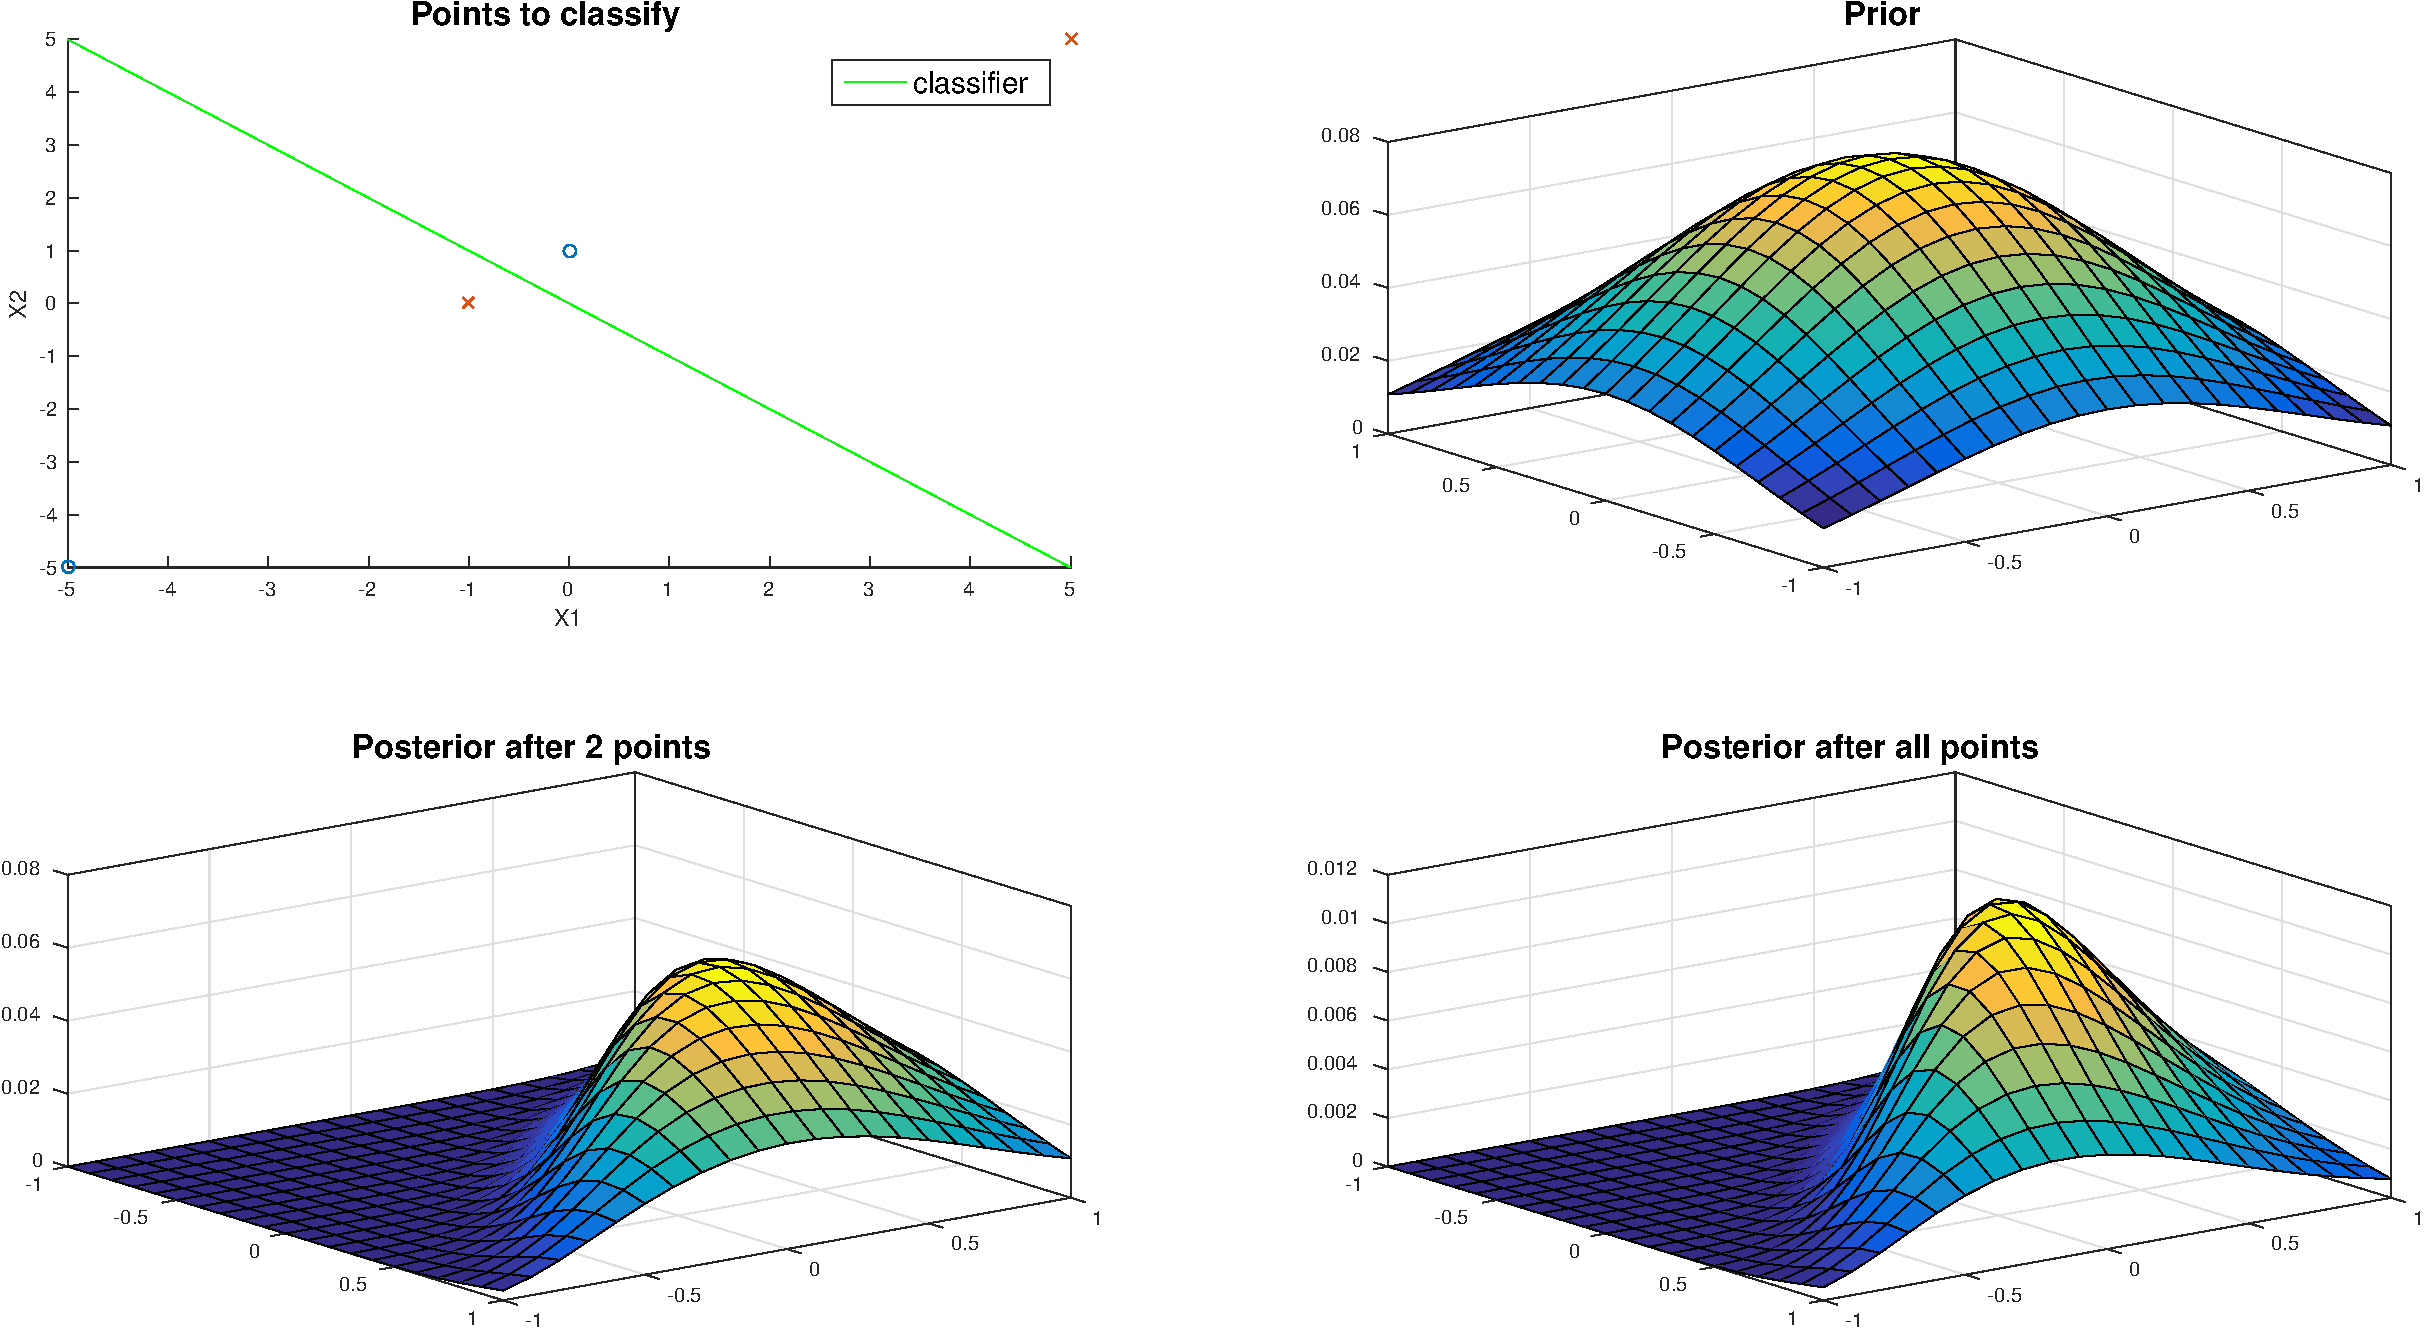
\includegraphics[scale=.40]{bayesnn.pdf}
    \caption{Bottom: evolution of the posterior through training. Top:
      in green, the classifier extracted using MAP on the weights'
      distribution}
    \label{fig:bayesnn}
\end{figure}

\section{Decision boundary of classifier}

\section{Function approximation}
\bibliographystyle{ieeetr} 
\bibliography{bib-db}

\end{document}
